%%%%%%%%%%%%%%%%%%%%%%%%%%%%%%%%%%%%%%%%%%%%%%%%%%%%%%%%%%%%%%%%%%%%%%
% Lớp 10 | Bất phương trình bậc 2 một ẩn | Phương trình quy về phương trình bậc hai
% Dạng 0D7?3-2: Phương trình căn
% Số câu: 42  (sinh tự động bởi tach_cau.py; từ nay thầy sửa trực tiếp file này)
%%%%%%%%%%%%%%%%%%%%%%%%%%%%%%%%%%%%%%%%%%%%%%%%%%%%%%%%%%%%%%%%%%%%%%

%%%%%%%%%%%%%%%% TRẮC NGHIỆM 4 PHƯƠNG ÁN %%%%%%%%%%%%%%%%

% nguồn: MaHoaNH_TracNghiem_Lop10
\begin{ex}%[0D7N3-2]%[ma:e67e072c]
	 Cho phương trình $\sqrt{3x+4} = x\quad (1)$. Mệnh đề nào sau đây đúng?
	 \choice
		 {$(1)\Leftrightarrow 3x+4=x^2$}
		 {$(1)\Leftrightarrow 3x+4=x$}
		 {$(1)\Leftrightarrow \heva{&3x+4\ge 0\\ &3x+4=x^2}$}
		{\True $(1)\Leftrightarrow \heva{&x\ge  0\\ &3x+4=x^2}$}
	 \loigiai{
		Ta có  $(1)\Leftrightarrow \heva{&x\ge 0\\ &3x+4=x^2}.$
	 }
\end{ex}

% nguồn: MaHoaNH_TracNghiem_Lop10
\begin{ex}%[0D7H3-2]%[ma:12dfe583]
	Nghiệm của phương trình  $\sqrt{2x-1}=x$ là
	\choice 
		 {$x=-1$}
		{$x=2$} 
		{\True  $x=1$}
		{$x=0$} 
	\loigiai{ 
		Phương trình $\sqrt{2x-1}=x\Rightarrow 2x-1=x^2\Leftrightarrow  x=1$.\\
		Thử lại  $x=1$ vào phương trình thấy thỏa mãn.
	 }
\end{ex}

% nguồn: MaHoaNH_TracNghiem_Lop10
\begin{ex}%[0D7H3-2]%[ma:b29c15ee]
	Tổng  tất cả các nghiệm của phương trình $\sqrt{x^2+5x-5}=2x-1$ bằng
	\choice 
		 {\True $3$}
		{$1$} 
		 {$-2$}
		{$-3$} 
	\loigiai{ Ta  có
		\[\sqrt{x^2+5x-5}=2x-1\Rightarrow x^2+5x-5=4x^2-4x+1\Rightarrow 3x^2-9x+6=0\Rightarrow  \hoac{&x=2\\&x=1.}\]
		Thay lần lượt $x=2$,  $x=1$ vào phương trình đã cho, ta thấy $x=2$, $x=1$ đều thỏa mãn.\\
		Do đó phương trình đã cho có nghiệm $x=2$,  $x=1$.\\
		Vậy tổng  các nghiệm của phương trình đã cho là $2+1=3$.
	 }
\end{ex}

% nguồn: MaHoaNH_TracNghiem_Lop10
\begin{ex}%[0D7H3-2]%[ma:3aac0742]
	 Số nghiệm của phương trình $\sqrt{3x^2 - 9x + 1} = |x-2|$ là
	 \choice
		 {$0$}
		{$1$} 
		{\True  $2$}
		 {$3$}
	\loigiai{ 
		Ta có phương trình tương đương với 
		 \[
		3x^2 - 9x + 1 = (x-2)^2 \Leftrightarrow 2x^2 - x - 21 = 0 \Leftrightarrow \hoac{&x=-3 \\ & x = \dfrac{7}{2}.} 
		 \]
		Vậy phương  trình có $2$ nghiệm.
	} 
\end{ex}

% nguồn: MaHoaNH_TracNghiem_Lop10
\begin{ex}%[0D7H3-2]%[ma:e371cb9d]
	Tập nghiệm $S$ của phương trình $\sqrt{x^2-4} =  x-2 $ là
	 \choice
		{$S =  \{0\}$}
		{\True $S  = \{2\}$}
		{$S =  \{0;2\}$}
		{$S = \emptyset$} 
	 \loigiai{
		Ta có phương trình  tương đương với
		\[ 
		\Leftrightarrow \heva{&x-2\ge 0\\ &x^2-4 = (x-2)^2} \Leftrightarrow \heva{&x\ge 2\\ &4x-8 = 0} \Leftrightarrow  x=2.
		\] 
		Vậy  tập nghiệm của phương trình là $S = \{2\}$.
	} 
\end{ex}

% nguồn: MaHoaNH_TracNghiem_Lop10
\begin{ex}%[0D7H3-2]%[ma:3abfdcf5]
	Tập nghiệm $S$ của phương trình $\sqrt{2x-3} = x-3  $ là
	 \choice
		{\True $S  = \{6\}$}
		{$S = \{2\}$} 
		{$S  = \{2;6\}$}
		{$S =  \emptyset$}
	\loigiai{ 
		Ta có  phương trình tương đương với
		\[ 
		\Leftrightarrow \heva{&x-3\ge 0\\ &2x-3  = (x-3)^2} \Leftrightarrow \heva{&x\ge 3\\ &x^2 - 8x + 12 = 0} \Leftrightarrow \heva{&x\ge 3\\ &\hoac{&x=2\\ &x=6}} \Leftrightarrow x=6.
		 \]
		Vậy tập nghiệm  của phương trình là $S = \{6\}$.
	 }
\end{ex}

% nguồn: MaHoaNH_TracNghiem_Lop10
\begin{ex}%[0D7H3-2]%[ma:c78dfccc]
	Nghiệm của phương trình $\sqrt{4x^2+2x+10}=3x+1$  là
	 \choice
		{\True  $x=1$}
		{ $x=\dfrac{-9}{5}$} 
		 {$\hoac{&x=\dfrac{-9}{5}\\&x=1}$}
		{$x\in\emptyset$} 
	\loigiai{Bình  phương hai vế của phương trình đã cho, ta được
		\begin{eqnarray*}
			4x^2+2x+10=(3x+1)^2  \Rightarrow -5x^2-4x+9=0\Rightarrow \hoac{&x=1\\ &x=-\dfrac{9}{5}.}
		\end{eqnarray*}
		Thay lần lượt các giá trị trên vào phương trình đã cho, ta thấy $x=1$ thỏa mãn.\\ 
		Vậy nghiệm của phương trình đã cho là $x=1$. 
	 }
\end{ex}

% nguồn: MaHoaNH_TracNghiem_Lop10
\begin{ex}%[0D7H3-2]%[ma:c42f53d5]
	Nghiệm của  phương trình $\sqrt{(x-1)(2x-1)}-2x-1=0$ là
	\choice 
		 {$x=-\dfrac{7}{2}$}
		 {\True $x=0$}
		{$\hoac{&x=0\\&x=-\dfrac{7}{2}}$} 
		 {$x\in\emptyset$}
	\loigiai{Phương trình  đã cho được viết lại $\sqrt{(x-1)(2x-1)}=2x+1$.\\
		Bình phương hai vế của phương  trình trên, ta được
		\begin{eqnarray*}
			 (x-1)(2x-1)=(2x+1)^2\Rightarrow -2x^2-7x=0\Rightarrow \hoac{&x=0\\ &x=-\dfrac{7}{2}.}
		\end{eqnarray*}
		Thay lần lượt các giá trị trên vào phương  trình đã cho, ta thấy $x=0$ thỏa mãn.\\
		Vậy nghiệm  của phương trình đã cho là $x=0$.
	} 
\end{ex}

% nguồn: MaHoaNH_TracNghiem_Lop10
\begin{ex}%[0D7H3-2]%[ma:d1750915]
	Tổng các nghiệm của phương trình $\sqrt{4+2x-x^2} = x-2$ là 
	 \choice
		 {$0$}
		{$1$} 
		 {$2$}
		 {\True $3$}
	\loigiai{ 
		Bình phương hai vế  của phương trình đã cho, ta được
		\begin{eqnarray*}
			4+2x-x^2=(x-2)^2\Rightarrow 4+2x-x^2=x^2-4x+4\Rightarrow 2x^2-6x=0\Rightarrow x=0 \ \text{hoặc}  \ x=3.
		\end{eqnarray*}
		Thay lần lượt các giá trị trên vào phương trình đã cho,  ta thấy $x=3$ thỏa mãn.\\
		 Vậy nghiệm của phương trình đã cho là $x=3$.
	 }
\end{ex}

% nguồn: MaHoaNH_TracNghiem_Lop10
\begin{ex}%[0D7H3-2]%[ma:283c45d2]
	Nghiệm của phương trình $x-\sqrt{3x^2-9x+1}=2$ là 
	\choice 
		{\True  $x=3$}
		{$x=-\dfrac{1}{2}$} 
		 {$\hoac{&x=-\dfrac{1}{2}\\&x=3}$}
		 {$x\in\emptyset$}
	\loigiai{Phương  trình đã cho được viết lại $\sqrt{3x^2-9x+1}=x-2$.\\
		Bình phương hai vế của  phương trình trên, ta được
		\begin{eqnarray*}
			 3x^2-9x+1=(x-2)^2\Rightarrow2x^2-5x-3=0\Rightarrow \hoac{&x=3\\ &x=\dfrac{1}{2}.}.
		\end{eqnarray*}
		Thay lần lượt các giá trị trên vào phương trình đã  cho, ta thấy $x=3$ thỏa mãn.\\
		Vậy nghiệm của phương trình đã cho là  $x=3$.
	} 
\end{ex}

% nguồn: MaHoaNH_TracNghiem_Lop10
\begin{ex}%[0D7H3-2]%[ma:140e9a89]
	 Tổng các nghiệm của phương trình $\sqrt{x^2-3x+2}=x-1$ là
	 \choice
		 {$0$}
		 {\True $1$}
		{$2$} 
		 {$3$}
	 \loigiai{
		 Bình phương hai vế của phương trình đã cho, ta được
		\begin{eqnarray*}
			 x^2-3x+2=(x-1)^2\Rightarrow x^2-3x+2=x^2-2x+1\Rightarrow -x+1=0\Rightarrow x=1.
		\end{eqnarray*}
		Thay $x=1$ vào phương trình đã cho, ta thấy $x=1$  thỏa mãn.\\
		Vậy nghiệm của phương  trình đã cho là $x=1$.
	} 
\end{ex}

% nguồn: MaHoaNH_TracNghiem_Lop10
\begin{ex}%[0D7H3-2]%[ma:ccca6b68]
	Tổng các  nghiệm của phương trình $\sqrt{2x-1} = x-2$ là
	 \choice
		{$6$} 
		 {$1$}
		 {\True $5$}
		 {$2$}
	 \loigiai{
		Ta có phương trình tương đương với 
		\[ 
		\heva{&x-2\ge  0\\ &2x-1 = (x-2)^2}
		\Leftrightarrow \heva{&x\ge 2\\ &x^2 - 6x + 5  = 0}
		\Leftrightarrow \heva{&x\ge 2\\ &\hoac{&x=1\\  &x=5}}
		\Leftrightarrow  x=5.
		 \]
	 }
\end{ex}

% nguồn: MaHoaNH_TracNghiem_Lop10
\begin{ex}%[0D7H3-2]%[ma:bfcbb47a]
	Tổng các nghiệm của phương trình $\sqrt{x^2+3} = 3x-1$ là 
	 \choice
		{$0$} 
		 {\True $1$}
		 {$2$}
		{$3$} 
	 \loigiai{
		Ta có phương  trình tương đương với
		\[ 
		\heva{&3x-1\ge 0\\  &x^2+3 = (3x-1)^2}
		\Leftrightarrow \heva{&x\ge  \dfrac{1}{3}\\ &8x^2-6x-2=0}
		\Leftrightarrow  \heva{&x\ge\dfrac{1}{3}\\ &\hoac{&x=1\\ &x=-\dfrac{1}{4}}}
		\Leftrightarrow  x=1.
		 \]
	 }
\end{ex}

% nguồn: MaHoaNH_TracNghiem_Lop10
\begin{ex}%[0D7H3-2]%[ma:2bac41c6]
	Số nghiệm của  phương trình $x - \sqrt{2x^2-3x+1} = 1$ là
	 \choice
		{$0$} 
		{$2$} 
		{$3$} 
		{\True  $1$}
	 \loigiai{
		Ta có phương trình tương đương với 
		 \[
		\heva{&x-1\ge 0\\ &2x^2-3x+1  = (x-1)^2}
		\Leftrightarrow \heva{&x\ge 1\\  &x^2-x=0}
		\Leftrightarrow \heva{&x\ge  1\\ &\hoac{&x=0\\ &x=1}}
		 \Leftrightarrow x=1.
		 \]
	} 
\end{ex}

% nguồn: MaHoaNH_TracNghiem_Lop10
\begin{ex}%[0D7H3-2]%[ma:f2cfedb2]
	Số nghiệm của phương  trình $\sqrt{-x^2 + 4x} = 2x-2$ là
	\choice 
		 {$0$}
		 {$2$}
		 {$3$}
		{\True $1$} 
	 \loigiai{
		Ta có phương trình tương đương với 
		 \[
		\heva{&2x-2\ge 0\\ &-x^2+4x  = (2x-2)^2}
		\Leftrightarrow \heva{&x\ge 1\\ &5x^2 - 12x +  4 = 0}
		\Leftrightarrow \heva{&x\ge 1\\  &\hoac{&x=2\\ &x=\dfrac{2}{5}}}
		\Leftrightarrow  x=2.
		\] 
	} 
\end{ex}

% nguồn: MaHoaNH_TracNghiem_Lop10
\begin{ex}%[0D7H3-2]%[ma:6dc9cfd5]
	Tập nghiệm của  phương trình $\sqrt{5x+6} = x-6$ là
	\choice 
		{$S=\{2\}$} 
		{$S  = \{6\}$}
		{$S  = \{2;15\}$}
		{\True  $S = \{15\}$}
	\loigiai{ 
		Ta có phương trình tương đương với 
		\[ 
		\heva{&x-6\ge  0\\ &5x+6 = (x-6)^2}
		\Leftrightarrow \heva{&x\ge 6\\  &x^2 - 17x + 30 = 0}
		\Leftrightarrow \heva{&x\ge 6\\ &\hoac{&x=2\\ &x=15}} 
		 \Leftrightarrow x=15.
		 \]
		Vậy tập nghiệm  của phương trình là $S = \{ 15 \}$.
	 }
\end{ex}

% nguồn: MaHoaNH_TracNghiem_Lop10
\begin{ex}%[0D7H3-2]%[ma:b1af6611]
	Số nghiệm của phương trình $\sqrt{3x^2 - 9x + 7} =  x - 2$ là
	\choice 
		{$3$} 
		 {$1$}
		{$2$} 
		{\True $0$} 
	 \loigiai{
		Ta có phương trình tương  đương với
		 \[
		 \heva{&x-2\ge 0\\ &3x^2 - 9x + 7 = (x-2)^2}
		\Leftrightarrow \heva{&x\ge 2\\ &2x^2 - 5x+3=0} 
		\Leftrightarrow \heva{&x\ge  2\\ &\hoac{&x=1\\ &x=\dfrac{3}{2}}}
		\Leftrightarrow  x\in \emptyset.
		 \]
		Vậy  phương trình vô nghiệm.
	} 
\end{ex}

% nguồn: MaHoaNH_TracNghiem_Lop10
\begin{ex}%[0D7H3-2]%[ma:bc382559]
	 Số nghiệm nguyên của phương trình $\sqrt{x^2 +10x-5} = 2(x-1)$ là
	\choice 
		{\True $0$} 
		{$2$} 
		 {$3$}
		 {$1$}
	 \loigiai{
		 Ta có phương trình tương đương với
		\[ 
		\heva{&2(x-1)\ge  0\\ &x^2+10x-5 = [2(x-1)]^2}
		\Leftrightarrow \heva{&x\ge  1\\ &3x^2 - 18x +9 = 0}
		\Leftrightarrow \heva{&x\ge  1\\ &x=3\pm 6}
		\Leftrightarrow x=3+\sqrt{6}. 
		\] 
		Vậy phương trình không  có nghiệm nguyên.
	 }
\end{ex}

% nguồn: MaHoaNH_TracNghiem_Lop10
\begin{ex}%[0D7H3-2]%[ma:c9408bda]
	Giải phương trình $\sqrt{x^2-4x+5}=x+3$ ta được nghiệm $x=\dfrac{a}{b}$ với $a\in\mathbb{Z}$, $b\in\mathbb{N}$ và $\dfrac{a}{b}$ là phân số tối giản. Tính $a+b$. 
	 \choice
		 {$4$}
		{\True $3$} 
		{$-3$} 
		{$-7$} 
	\loigiai{ 
		Ta có $x^2-4x+5=\left(x-2\right)^2+1>0, \forall  x\in\mathbb{R}$.
		\begin{eqnarray*}
			& &  \sqrt{x^2-4x+5}=x+3\\
			&\Rightarrow  & x^2-4x+5=\left(x+3\right)^2\\
			&\Rightarrow  & x^2-4x+5=x^2+6x+9\\
			&\Rightarrow  & 10x=-4\\
			&\Rightarrow  & x=\dfrac{-2}{5}.
		\end{eqnarray*}
		Thử  lại $x=\dfrac{-2}{5}$ vào phương trình $\sqrt{x^2-4x+5}=x+3$ ta thấy thỏa mãn.\\
		Vậy  $a+b=-2+5=3$.
	} 
\end{ex}

% nguồn: MaHoaNH_TracNghiem_Lop10
\begin{ex}%[0D7H3-2]%[ma:6b547bcc]
	Tổng các  nghiệm của phương trình $\sqrt{2x^2+x-6}=x+2$ là
	 \choice
		 {$5$}
		 {$-2$}
		 {$-3$}
		{\True $3$} 
	 \loigiai{
		 Bình phương hai vế phương trình ta được
		\allowdisplaybreaks 
		\begin{eqnarray*}
			 &&2x^2+x-6=(x+2)^2
			\\ 
			&\Leftrightarrow&2x^2+x-6=x^2+4x+4 
			 \\
			 &\Leftrightarrow&x^2-3x-10=0
			 \\
			&\Leftrightarrow&\hoac{&x=5\\&x=-2.} 
		\end{eqnarray*}
		Thử lại, $x=5$ và $x=-2$ đều thỏa phương trình.\\ 
		Do đó phương trình có hai nghiệm là $\hoac{&x=5\\&x=-2.}$\\ 
		 Vậy tổng hai nghiệm là $5+(-2)=3$.
	} 
\end{ex}

% nguồn: MaHoaNH_TracNghiem_Lop10
\begin{ex}%[0D7B3-2]%[ma:bd8486ef]
	Biết phương trình $\sqrt{6x^2 +7x -1} = \sqrt{-29x^2 -41x + 10}$ có hai nghiệm $x_1; x_2$. Tính giá trị của biểu thức  $S=x_1x_2 + 2(x_1 +x_2)$
	\choice 
		 {$-\dfrac{96}{35}$}
		{$-\dfrac{11}{35}$} 
		{\True  $-\dfrac{107}{35}$}
		 {$\dfrac{85}{35}$}
	\loigiai{ 
		Điều kiện: $\heva{&6x^2 +7x  -1 \geq 0 \\& -29x^2 -41x + 10.}$\\
		Bình phương hai vế, phương trình  đã cho trở thành:\\
		$$6x^2 +7x -1 = -29x^2 -41x +10 \Leftrightarrow  35x^2 +48x -11=0.$$
		 Vì phương trình đã cho có hai nghiệm $x_1; x_2$ nên áp dụng định lí Vi-ét, ta được:
		$$\heva{&x_1  +x_2 = -\dfrac{48}{35} \\& x_1 x_2 = -\dfrac{11}{35}}$$
		Suy ra $S=x_1x_2 + 2(x_1 +x_2) = -\dfrac{11}{35} +2\cdot\left( -\dfrac{48}{35}  \right) = -\dfrac{107}{35}$.
	 }
\end{ex}


%%%%%%%%%%%%%%%% ĐÚNG/SAI %%%%%%%%%%%%%%%%

% nguồn: MaHoaNH_DungSai_Lop10
\begin{ex}%[0D7N3-2]%[ma:1916cc3f]
	Cho phương trình  $\sqrt{5x-4}=x$.
	\choiceTF 
		{Phương trình có một nghiệm} 
		 {Phương trình vô nghiệm}
		{\True  $x=1$ là nghiệm của phương trình}
		{\True $x=4$  là nghiệm của phương trình}
	 \loigiai{
		 Bình phương hai vế của phương trình $\sqrt{5x-4}=x$ ta được
		\begin{eqnarray*}
			&& 5x-4=x^2\\ 
			&\Leftrightarrow&  x^2-5x+4=0\\
			&\Leftrightarrow&  \hoac{&x=1\\&x=4.}
		\end{eqnarray*}
		Thay lần lượt các giá trị trên của $x$ vào phương trình ta thấy cả hai đều thỏa mãn.\\ 
		Vậy phương trình có nghiệm là $x=1$, $x=4$. 
	 }
\end{ex}

% nguồn: MaHoaNH_DungSai_Lop10
\begin{ex}%[0D7H3-2]%[ma:3d3b3ff0]
	Cho  phương trình $\sqrt{2x^2-5x+11}=x+1$.
	 \choiceTF
		 {\True Phương trình có hai nghiệm phân biệt}
		{Phương trình có một  nghiệm}
		{\True $x=2$ là nghiệm của phương  trình}
		{\True $x=5$ là nghiệm  của phương trình}
	\loigiai{ 
		Bình phương hai vế  của phương trình $\sqrt{2x^2-5x+11}=x+1$ ta được
		\begin{eqnarray*}
			 && 2x^2-5x+11=(x+1)^2\\
			&\Leftrightarrow& 2x^2-5x+11=x^2+2x+1\\ 
			 &\Leftrightarrow& x^2-7x+10=0\\
			&\Leftrightarrow&  \hoac{&x=2\\&x=5.}
		\end{eqnarray*}
		Thay lần lượt các giá trị  trên của $x$ vào phương trình ta thấy cả hai đều thỏa mãn.\\
		Vậy phương trình có nghiệm  là $x=2$, $x=5$.
	 }
\end{ex}

% nguồn: MaHoaNH_DungSai_Lop10
\begin{ex}%[0D7H3-2]%[ma:6c537a57]
	Cho phương trình $\sqrt{2x^2+x+3}=-x-5$~~$(*)$.  Khi đó
	 \choiceTF
		{\True Bình phương hai  vế của phương trình ta được $x^2-9x-22=0$}
		{Phương trình $\sqrt{2x^2+x+3}=-x-5$ và phương trình $x^2-9x-22=0$ có  chung tập nghiệm}
		{$x=11$; $x=-2$ là nghiệm của phương  trình $(*)$}
		{\True Tập nghiệm  của phương trình $(*)$ là $S=\varnothing$}
	 \loigiai{
		Ta có $\sqrt{2x^2+x+3}+x+5=0 \Leftrightarrow  \sqrt{2x^2+x+3}=-x-5$.\\
		Bình phương hai vế của phương trình, ta  được\\
		 \centerline{$2x^2+x+3=x^2+10x+25 \Rightarrow x^2-9x-22=0 \Rightarrow x=11$ hoặc $x=-2$.}\\
		Thay lần lượt $x=11$; $x=-2$ vào phương trình đã cho, ta thấy hai giá trị này  đều không thỏa mãn. Do đó, phương trình đã cho vô nghiệm.\\
		Vậy tập nghiệm của phương trình đã cho  là $S=\varnothing$.
		\begin{itemchoice}
			\itemch Bình  phương hai vế của phương trình ta được $x^2-9x-22=0$.
			\itemch Phương trình $\sqrt{2x^2+x+3}=-x-5$  có tập nghiệm là $S=\varnothing$, phương trình $x^2-9x-22=0$ có tập nghiệm $S=\{-2;11\}$.
			\itemch Ta có $x=11$; $x=-2$ là  nghiệm của phương trình $x^2-9x-22=0$.
			\itemch Tập nghiệm của phương trình $(*)$  là $S=\varnothing$.
		\end{itemchoice}
	} 
\end{ex}

% nguồn: MaHoaNH_DungSai_Lop10
\begin{ex}%[0D7H3-2]%[ma:3147f0c9]
	Cho phương trình $\sqrt{2x^2+x+3}=-x-5$ (*). Xét tính Đúng/Sai của các khẳng định  sau
	\choiceTF 
		{Phương trình $\sqrt{2x^2+x+3}=-x-5$ và phương trình $x^2-9x-22=0$ có cùng tập nghiệm} 
		{$x=0$ là nghiệm của phương trình (*)} 
		{\True Bình phương  hai vế của phương trình và thu gọn, ta được $x^2-9x-22=0$}
		{\True  Phương trình (*) vô nghiệm}
	\loigiai{ 
		Từ phương trình $\sqrt{2x^2+x+3}=-x-5$. Bình phương hai  vế của phương trình, ta được
		 $$
		2x^2+x+3=x^2+10x+25 \Rightarrow x^2-9x-22=0 \Rightarrow x=11 \text { hoặc  } x=-2
		 $$
		Thay lần lượt $x=11$; $x=-2$ vào phương trình đã cho, ta thấy hai giá trị này đều không thỏa mãn. Do  đó, phương trình đã cho vô nghiệm.\\
		Dựa vào kết quả trên ta có các kết luận 
		\begin{itemchoice}
			\itemch  Khẳng định sai.
			\itemch Thay $x=0$ vào phương trình ta được $\sqrt{3}=-5$ (không đúng). Vậy $x=0$  không là nghiệm của phương trình.\\
			 Khẳng định sai.
			\itemch Khẳng định đúng. 
			\itemch Khẳng định  đúng.
		\end{itemchoice}
	} 
\end{ex}

% nguồn: MaHoaNH_DungSai_Lop10
\begin{ex}%[0D7H3-2]%[ma:77a45bfb]
	Cho phương trình $\sqrt{2x^2+x+3}=-x-5$ (*). Xét tính Đúng/Sai của các khẳng định  sau
	\choiceTF 
		{$x=0$ là nghiệm của phương trình (*)} 
		{\True Bình phương hai vế  của phương trình và thu gọn, ta được $x^2-9x-22=0$}
		 {Phương trình $\sqrt{2x^2+x+3}=-x-5$ và phương trình $x^2-9x-22=0$ có cùng tập nghiệm}
		{\True Phương trình (*) vô nghiệm} 
	 \loigiai{
		Từ phương trình $\sqrt{2x^2+x+3}=-x-5$. Bình phương hai vế  của phương trình, ta được
		$$ 
		2x^2+x+3=x^2+10x+25 \Rightarrow x^2-9x-22=0 \Rightarrow x=11  \text { hoặc } x=-2
		 $$
		Thay lần lượt $x=11$; $x=-2$ vào phương trình đã cho, ta thấy hai giá trị  này đều không thỏa mãn. Do đó, phương trình đã cho vô nghiệm.\\
		Dựa vào kết quả trên  ta có các kết luận
		\begin{itemchoice}
			\itemch Thay $x=0$ vào phương trình ta  được $\sqrt{3}=-5$ (không đúng). Vậy $x=0$ không là nghiệm của phương trình.\\
			 Khẳng định sai.
			\itemch Khẳng định đúng. 
			\itemch Khẳng định sai. 
			\itemch Khẳng  định đúng.
		\end{itemchoice}
	} 
\end{ex}

% nguồn: MaHoaNH_DungSai_Lop10
\begin{ex}%[0D7V3-2]%[ma:ce1b6866]
	Cho phương trình $\sqrt{2x^2 + x+ 3} =  -(x+5)\quad (1)$. Khi đó
	\choiceTF 
		{\True Bình phương hai vế của phương trình $(1)$ ta được phương trình  $x^2 - 9x - 22 = 0$}
		{Phương  trình $(1)$ cùng tập nghiệm với phương trình $x^2 - 9x - 22 = 0$}
		{$x=11$ và $x=-2$ là  hai nghiệm của phương trình $(1)$}
		{\True Phương  trình $(1)$ vô nghiệm}
	\loigiai{ 
		Bình phương hai vế của  phương trình $(1)$ ta được
		\[ 
		2x^2 + x + 3 = (x+5)^2 \Leftrightarrow x^2 - 9x - 22 = 0 \Leftrightarrow \hoac{&x=11\\ & x  = -2.}
		 \]
		Thử lại ta thấy cả $x=11$ và $x=-2$ đều không thoả mãn. Vậy 
		\begin{itemchoice}
			\itemch Bình phương hai vế và thu gọn ta được phương trình $x^2  - 9x - 22 = 0$.
			\itemch Phương trình $(1)$ vô nghiệm mà tập nghiệm của phương trình $x^2 - 9x - 22 = 0$  là $S = \{ -2;11 \}$.
			\itemch  Phương trình đã cho vô nghiệm.
			\itemch Phương trình $(1)$ vô  nghiệm.
		\end{itemchoice}
	} 
\end{ex}

% nguồn: MaHoaNH_DungSai_Lop10
\begin{ex}%[0D7V3-2]%[ma:ec08b1cd]
	Cho phương trình $\sqrt{2x^2 +  x - 6} = x+2\quad (1)$. Khi đó
	 \choiceTF
		{Bình phương hai vế của phương trình $(1)$ ta được phương trình $x^2 + 3x  - 10 = 0$}
		{Điều kiện  xác định của phương trình là $x\ge 3$}
		{\True Phương trình $(1)$ có hai nghiệm  phân biệt}
		 {\True Tổng các nghiệm của phương trình $(1)$ là $3$}
	 \loigiai{
		Bình phương hai vế của phương trình $(1)$ ta được 
		 \[
		2x^2 + x - 6 = (x+2)^2 \Leftrightarrow x^2 - 3x - 10 = 0 \Leftrightarrow \hoac{&x=5\\ & x  = -2.}
		\] 
		Thử lại  ta thấy $x=5$ và $x=-2$ đều thoả mãn. Vậy
		\begin{itemchoice}
			\itemch Bình phương hhai vế và thu gọn, ta được  phương trình $x^2 - 3x - 10 = 0$.
			 \itemch Phương trình xác định khi và chỉ khi
			\[ 
			 2x^2 + x - 6 \ge 0 \Leftrightarrow (x+2)(x-3)\ge 0 \Leftrightarrow \hoac{&x\ge 3\\ &x\le -2.}
			\] 
			\itemch Phương trình có hai nghiệm $-2$ và $5$. 
			\itemch  Ta có tổng các nghiệm là $5 + (-2) = 3$.
		\end{itemchoice}
	} 
\end{ex}

% nguồn: MaHoaNH_DungSai_Lop10
\begin{ex}%[0D7V3-2]%[ma:5b619a6f]
	Cho  phương trình $\sqrt{-x^{2}+13x-2m-12}=\sqrt{-2x^{2}+10x-8}$.
	 \choiceTF
		{\True Với $m=1$ thì bình phương hai vế phương trình đã cho ta  được $x^{2}+3x-6=0$}
		{Có đúng một giá trị nguyên của tham  số $m$ để phương trình đã chocó nghiệm}
		{Phương trình đã cho có nghiệm khi $m\in[a;b]$, khi đó  $a+b=8$}
		{\True Giá trị nguyên lớn nhất của tham số  $m$ để phương trình đã cho có nghiệm là $12$}
	\loigiai{ 
		\begin{itemchoice}
			\itemch  Ta có
			\begin{eqnarray*}
				 &&\sqrt{-x^{2}+13x-2m-12}=\sqrt{-2x^{2}+10x-8}\\
				&\Leftrightarrow&\heva{&-2x^{2}+10x-8\geq  0\\&x^{2}+3x-4=2m}\\
				&\Leftrightarrow&\heva{&1\leq x\leq  4\\&x^{2}+3x-4=2m.\quad (1)}
			\end{eqnarray*}
			Với $m=1$ thì bình phương hai vế  phương trình đã cho ta được $x^{2}+3x-6=0$.
			\itemch Để phương trình đã  cho có nghiệm thì phương trình ($1$) có nghiệm thuộc đoạn $[1;4]$\\
			Số nghiệm  của phương trình ($1$) là số giao điểm của đồ thị hàm số $y=x^{2}+3x-4$ và đường thẳng $y=2m$.\\
			 Xét hàm số $y=x^{2}+3x-4$ có đồ thị như hình vẽ
			\begin{center}
				\begin{tikzpicture}[scale=0.4,font=\footnotesize,line join=round,line cap=round,>=stealth]
						\def \xmin{-4.5} 
						 \def \xmax{3.5}
						 \def \ymin{-7}
						\def \ymax{1.5} 
						\draw[->]  (\xmin,0)--(\xmax,0) node[shift=(-110:0.2)] {$x$};
						\draw[->] (0,\ymin)--(0,\ymax) node[shift=(-150:0.2)]  {$y$};
						 \fill (0,0) circle (1pt) node[shift=(-135:0.25)]{$O$}
						(-3/2,0)  circle (1pt) node[shift=(90:0.3)]{$-\tfrac{3}{2}$}
						 (0,-25/4) circle (1pt) node[shift=(0:0.4)]{$-\tfrac{25}{4}$};
						\draw[dashed]  (-3/2,0)|-(0,-25/4);
						\clip (\xmin,\ymin) rectangle (\xmax,\ymax); 
						\draw[smooth,samples=100,domain=\xmin:\xmax] plot  (\x,{(\x)^2+3*(\x)-4});
					\end{tikzpicture}
			\end{center}
			Dựa vào đồ thị hàm số, để phương trình đã cho có nghiệm thuộc đoạn $[1;4]$ thì $m\in[0;12]$.\\ 
			Có tất cả $13$ giá trị nguyên của tham số $m$ để phương trình đã  cho có nghiệm.
			\itemch Phương trình đã cho có nghiệm khi  $m\in[a;b]$, khi đó $a+b=12$.
			\itemch Giá trị nguyên lớn nhất của tham số $m$ để phương trình đã  cho có nghiệm là $12$.
		\end{itemchoice}
	} 
\end{ex}


%%%%%%%%%%%%%%%% TRẢ LỜI NGẮN %%%%%%%%%%%%%%%%

% nguồn: MaHoaNH_TraLoiNgan_Lop10
\begin{bt}%[0D7H3-2]%[ma:97d9a2b1]
	Tính  tổng bình phương tất cả các nghiệm của phương trình $\sqrt{3x^2+5x-13}=x+1$. \shortans{4}
	\loigiai{ Ta có 
		\[\sqrt{3x^2+5x-13}=x+1\Rightarrow 3x^3+5x-13=(x+1)^2\Rightarrow 2x^2+3x-14=0\Rightarrow x=2\ \text{hoặc}  \ x=-\dfrac{7}{2}.\]
		Thay lần lượt $x=2$, $  x=-\dfrac{7}{2}$ vào phương trình đã cho ta thấy chỉ có $x=2$ thỏa mãn.\\
		Vậy nghiệm duy nhất của phương trình  đã cho là $x=2$ và $2^2=4$.
	} 
\end{bt}

% nguồn: MaHoaNH_TraLoiNgan_Lop10
\begin{bt}%[0D7H3-2]%[ma:b4e37fc4]
	Nghiệm của phương trình $\sqrt{2 x^2-5 x-9}=x-1$  bằng bao nhiêu?
	 \shortans{5}
	\loigiai{ 
		Điều  kiện $x \geq 1$.
		Bình phương hai vế của phương trình ta được 
		 $$
		2  x^2-5 x-9=x^2-2 x+1 \Leftrightarrow x^2-3 x-10=0 \Leftrightarrow\hoac{
		 &x=5 \\
		&x=-2.}$$ 
		Đối chiếu với điều kiện $x \geq 1$ ta  thấy chỉ có $x=5$ thỏa mãn.\\
	 Vậy nghiệm của phương trình đã cho là $x=5$.}
\end{bt}

% nguồn: MaHoaNH_TraLoiNgan_Lop10
\begin{bt}%[0D7H3-2]%[ma:5aea71a4]
	Gọi $S$  là tập nghiệm của phương trình $\sqrt{3x^2+5x-6}=x+3$. Tìm số phần tử của $S$.
	 \shortans{2}
	 \loigiai{
		Ta  có
		\begin{eqnarray*}
			 && \sqrt{3x^2+5x-6}=x+3 \\
			 &\Rightarrow & 3x^2+5x-6=x^2+6x+9\\
			&\Rightarrow& 2x^2-x-15=0  \\
			 &\Rightarrow& \hoac{&x=3\\&x=-\dfrac{5}{2}.}
		\end{eqnarray*}
		 Thử lại nhận $x=3$, $x=-\dfrac{5}{2}$.\\
		Vậy tập nghiệm phương trình là  $S=\left\{ 3; -\dfrac{5}{2}\right\}$.
	} 
\end{bt}

% nguồn: MaHoaNH_TraLoiNgan_Lop10
\begin{bt}%[0D7H3-2]%[ma:342e8771]
	Tính tổng  tất cả các nghiệm của phương trình $\sqrt{3x^2-2x+16}+1=2x$.
	 \shortans{5}
	\loigiai{ 
		 Điều kiện: $3x^2-2x+16\geq0$.\\
		 Ta có $\sqrt{3x^2-2x+16}+1=2x\Leftrightarrow \sqrt{3x^2-2x+16}=2x-1$.\\
		Bình phương hai vế phương trình, ta được 
		\begin{eqnarray*}
			&&3x^2-2x+16=(2x-1)^2\\ 
			&\Rightarrow&3x^2-2x+16=4x^2-4x+1\\ 
			&\Rightarrow&-x^2+2x+15=0\\ 
			&\Rightarrow&\hoac{&x=-3\\&x=5.} 
		\end{eqnarray*}
		Thử  lại, ta thay các giá trị $x=5$, $x=-3$ vào phương trình đã cho, ta thấy chỉ có giá trị $x=5$ thỏa mãn.\\
		Vậy phương trình  đã có có nghiệm $x=5$.\\
		Tổng tất cả các nghiệm của phương  trình là $5$.
	 }
\end{bt}

% nguồn: MaHoaNH_TraLoiNgan_Lop10
\begin{bt}%[0D7H3-2]%[ma:393b3a7c]
	Tính tổng bình phương tất cả các nghiệm của phương  trình $x\sqrt{x^2+x+2}=2x$.
	 \shortans{53}
	 \loigiai{
		 \allowdisplaybreaks
		$\begin{aligned}
		x\sqrt{x^2+x+2}=2x\Leftrightarrow x\cdot(\sqrt{x^2+x+2}-2)=0\Leftrightarrow\hoac{&x=0\\&\sqrt{x^2+x+2}=2.\quad(1)} 
	\end{aligned}$\\
	Bình phương hai vế của phương trình $(1)$ ta  được
	$$x^2+x+2=4\Leftrightarrow  x^2+x-2=0\Leftrightarrow \hoac{&x=1\\&x=-2.}$$
	Thử lại: 
	\begin{itemize}
		 \item $x=0$ thỏa mãn phương trình.
		 \item $x=1$ thỏa mãn phương trình.
		 \item $x=-2$ thỏa mãn phương trình.
	\end{itemize}
	Khi đó tổng bình  phương các nghiệm là $0+1+4=5$.
 }
\end{bt}


%%%%%%%%%%%%%%%% TỰ LUẬN %%%%%%%%%%%%%%%%

% nguồn: MaHoaNH_TuLuan_Lop10
\begin{bt}%[0D7V3-2]%[ma:d1f65647]
	Giải phương  trình $\sqrt{2x^2+21x+55}=x+7$.
	 \loigiai{
		Xét phương trình $\sqrt{2x^2+21x+55}=x+7$\ \ \ $(1)$.\\ 
		Bình phương  hai vế của phương trình ta được
		 $$2x^2+21x+55=(x+7)^2\Leftrightarrow x^2+7x+6=0\Leftrightarrow\hoac{&x=-1\\&x=-6.}$$
		Thử lại ta thấy $x=-1$ và $x=-6$  đều thỏa mãn phương trình.\\
		 Vậy phương trình có 2 nghiệm $x=-1$ và $x=-6$.
	} 
\end{bt}

% nguồn: MaHoaNH_TuLuan_Lop10
\begin{bt}%[0D7C3-2]%[ma:6ecd3e46]
	Tính tổng các nghiệm của phương trình $\sqrt{x^2 - 4x - 1} -  |2x+1| = 1$.
	 \loigiai{
		Ta xét hai trường  hợp:
		\begin{enumerate}[\bf TH1.]
			\item  $2x+1\ge 0 \Leftrightarrow x \ge -\dfrac{1}{2}$.\\
			Khi đó  phương trình trở thành
			\begin{eqnarray*}
				& &\sqrt{x^2 - 4x - 1} - (2x+1) =  1 \Leftrightarrow \sqrt{x^2 - 4x - 1} = 2x+2\\
				& \Leftrightarrow & \heva{&2x+2\ge 0\\ &x^2  - 4x - 1 = (2x+2)^2}
				\Leftrightarrow  \heva{&x\ge -1\\ &3x^2 + 12x + 5 = 0}\\
				 &\Leftrightarrow &\heva{&x\ge -1\\ &x = \dfrac{-6\pm \sqrt{21}}{3}}
				\Leftrightarrow x =  \dfrac{-6+\sqrt{21}}{3} \text{ (thoả mãn)}.
			\end{eqnarray*}
			\item $2x+1< 0 \Leftrightarrow  x < -\dfrac{1}{2}$. Khi đó phương trình trở thành
			\begin{eqnarray*}
				& &\sqrt{x^2 - 4x - 1} + (2x+1) =  1 \Leftrightarrow \sqrt{x^2 - 4x - 1} = -2x\\
				& \Leftrightarrow & \heva{&-2x\ge 0\\ &x^2 -  4x - 1 = (-2x)^2}
				\Leftrightarrow \heva{&x\le 0\\  &3x^2 + 4x + 1 = 0}\\
				&\Leftrightarrow &\heva{&x\le 0\\  &\hoac{&x=-1\\ &x=-\dfrac{1}{3}}}
				 \Leftrightarrow \hoac{&x=-1\\ &x=-\dfrac{1}{3}.}
			\end{eqnarray*}
			Mà $x<  -\dfrac{1}{2}$ nên $x=-1$.
		\end{enumerate}
		Tổng  các nghiệm của phương trình là $\dfrac{-6+\sqrt{21}}{3} + (-1) = \dfrac{-9+\sqrt{21}}{3}$.
	} 
\end{bt}

% nguồn: MaHoaNH_TuLuan_Lop10
\begin{bt}%[0D7B3-2]%[ma:071b4772]
	Giải phương trình $  \sqrt{3x^2-5x-1}=x-1 $
	\loigiai{ 
		Ta có  \allowdisplaybreaks
		\begin{eqnarray*}
			\sqrt{3x^2-5x-1}=x-1 &\Rightarrow&  3x^2-5x-1=x^2-2x+1\\
			&\Leftrightarrow&  2x^2-3x-2=0 \Leftrightarrow \hoac{& x=2 \\ & x=-\dfrac{1}{2}.}
		\end{eqnarray*}
		Thay lần lượt $ x=2 $ và $ x=-\dfrac{1}{2} $ vào phương trình đã cho ta thấy $ x=2 $ là nghiệm  của phương trình.
	 }
\end{bt}

% nguồn: MaHoaNH_TuLuan_Lop10
\begin{bt}%[0D7B3-2]%[ma:804556f6]
	 Giải phương trình $\sqrt{2x^{2}-5x+2}=x-2$.
	\loigiai{ 
		Ta  có
		 \allowdisplaybreaks
		$\begin{aligned}
		&\quad \sqrt{2x^{2}-5x+2}=x-2 &\Leftrightarrow \heva{&x-2\ge  0\\&2x^{2}-5x+2=(x-2)^{2}}\\
		&\Leftrightarrow \heva{&x\ge 2\\&x^{2}-x-2=0} &\Leftrightarrow \heva{&x\ge 2\\&x=-1;\, x=2} \Leftrightarrow  x=2.
	\end{aligned}$\\
	Vậy  phương trình có nghiệm $x=2$.
 }
\end{bt}

% nguồn: MaHoaNH_TuLuan_Lop10
\begin{bt}%[0D7Y3-2]%[ma:d6748f42]
	Giải phương trình  $\sqrt{8-2x} = 2x-6$.
	 \loigiai{
		 Ta có
		 \allowdisplaybreaks
		\begin{eqnarray*}
			 \sqrt{8-2x} = 2x-6 &\Rightarrow& 8-2x = (2x-6)^2 \\
			&\Rightarrow&  4x^2-22x+28=0 \\
			&\Rightarrow& \hoac{&x=2  \\ &x=\dfrac{7}{2}}
		\end{eqnarray*}
		Thay lần lượt các giá trị $x=2$ và $x=\dfrac{7}{2}$ vào phương trình đã cho,  ta nhận $x=\dfrac{7}{2}$ và loại $x=2$.\\
		Vậy $S=\left\{  \dfrac{7}{2} \right\}$.
	 }
\end{bt}

% nguồn: MaHoaNH_TuLuan_Lop10
\begin{bt}%[0D7K3-2]%[ma:82e52d61]
	 \immini
	 {
	Mặt cắt đứng của cột cây số trên quốc lộ có dạng nửa hình tròn ở phía trên và phía  dưới có dạng hình chữ nhật (xem hình bên). Biết rằng đường kính của nửa hình tròn cũng là cạnh trên của hình chữ nhật và đường chéo của hình chữ nhật có độ dài là $ 66 $ cm. Tính kích thước của hình chữ nhật, biết diện tích của phần hình chữ nhật bằng $\dfrac{10}{3}$ diện tích của phần nửa hình tròn. Lấy $ \pi =3{,}14$ và làm tròn kết quả đến số thập phân thứ $ 2 $.
	 }
	 {
	\begin{tikzpicture}[line join = round,line cap = round,>=stealth,thick,scale=1]
			\coordinate  (A) at (0,0);
			\coordinate (B)  at (-3.5,0);
			\coordinate (C) at (-3.5,-4.5); 
			\coordinate  (D) at (0,-4.5);
			 \draw (A) arc (0:180:1.75cm);
			\draw (A)--(B)--(C)--(D)--cycle (A)--(C); 
			\path  (0.5,0)--(-3,-4.5) node[midway,align=center,sloped]{$ 66 $ cm};
			\draw (-2,-5); node{\text{mặt cắt của cột  cây số}};
		\end{tikzpicture}
	 }
	 \loigiai{
		Gọi $ x ~\mathrm{cm}~(x> 0)$ là đường kính của đường tròn.\\ 
		Ta có diện tích của phần hình chữ nhật là  $ x\cdot\sqrt{66^2-(x)^2} ~ \mathrm{cm^2} $.\\
		Diện tích của phần nửa hình tròn là $\dfrac{1}{2}\cdot \pi\cdot \left(\dfrac{x}{2}\right)^2=\dfrac{1}{8}\cdot  \pi x^2~ \mathrm{cm^2}$.\\
		Theo đề bài ta có \begin{eqnarray*}
		x\cdot\sqrt{66^2-(x)^2}  =\dfrac{10}{3}\cdot\dfrac{1}{8}\cdot \pi x^2&\Leftrightarrow &\sqrt{66^2-(x)^2} =\dfrac{5}{12}\cdot 3{,}14 \cdot x\\
		&\Leftrightarrow& \left(\dfrac{25}{144}\cdot 3{,}14^2+1\right)x^2=4356\\ 
		&  \Leftrightarrow& x \approx 40{,}08 .
	\end{eqnarray*}
	Vậy kích thước của hình chữ nhật là $ 2\left(40{,}08+ \sqrt{66^2-(40{,}08)^2}\right) \approx 185{,}03 ~\mathrm{cm}  $.
} 
\end{bt}

% nguồn: MaHoaNH_TuLuan_Lop10
\begin{bt}%[0D7K3-2]%[ma:c5c56730]
	Cho tam giác $ABC$ vuông tại $A$ có $AB$ ngắn hơn  $AC$ là $2\,\mathrm{cm}$, đặt $A B=x\, \mathrm{cm} $.
	\begin{listEX}
		\item Biểu diễn độ dài cạnh huyền  $BC$ theo $x$.
		\item Biết chu vi của tam giác $ABC$  là $24\,\mathrm{cm}$. Tìm độ dài $3$ cạnh của tam giác đó.
	\end{listEX}
	\loigiai{ 
		\begin{listEX}
			\item Gọi $A B=x \Rightarrow A C=x+2$.\\ 
			 Ta có tam giác $ABC$ vuông tại $A$ nên
			\allowdisplaybreaks{ 
			\begin{eqnarray*}
				&& BC^2 =  AB^2+AC^2 \\
				&\Leftrightarrow& BC^2 =  x^2+(x+2)^2 \\
				&\Rightarrow&  BC = \sqrt{2x^2+4x+4}.
			\end{eqnarray*}
			} 
			\item Ta có chu vi tam giác $ABC$ bằng  $24$ nên
			 \allowdisplaybreaks{
			\begin{eqnarray*}
				&&  A B+A C+B C=24\\
				&\Leftrightarrow& x+x+2+\sqrt{2x^2+4x+4}=24\\ 
				&\Leftrightarrow&  \sqrt{2x^2+4x+4}=22-2x\\
				&\Leftrightarrow& -2 x^2+92 x-480=0\\ 
				 &\Leftrightarrow& \hoac{&x=6 \\&x=40.}
			\end{eqnarray*}
			} 
			Thử lại, nhận $x=6$, loại  $x=40$.\\
			 Vậy độ dài ba cạnh là $AB=6$ cm, $AC=8$ cm và $B C=10$ cm.
		\end{listEX}
	} 
\end{bt}

% nguồn: MaHoaNH_TuLuan_Lop10
\begin{bt}%[0D7B3-2]%[ma:33e1f5db]
	Giải các  phương trình sau
	\begin{enumEX}[a)]{2}
		\item  $\sqrt{5-3x+x^2}=\sqrt{1-4x+4x^2}$.
		 \item $-3x+1=\sqrt{4x^2+4x}$.
	\end{enumEX}
	\loigiai{ 
		\begin{enumEX}[a)]{1}
			 \item $\sqrt{5-3x+x^2}=\sqrt{1-4x+4x^2}$\\
			Bình phương hai vế  của phương trình, ta được
			\allowdisplaybreaks 
			$$\begin{aligned}
			&5-3x+x^2=1-4x+4x^2\Rightarrow&3x^2-x-4=0\Rightarrow&\hoac{&x=-1\\&x=\dfrac{4}{3}.} 
		\end{aligned}$$
		 Thử lại:
		\begin{itemize}
			\item $x=-1$ thỏa mãn  phương trình.
			 \item $x=\dfrac{4}{3}$ thỏa mãn phương trình.
		\end{itemize}
		Vậy tập nghiệm  của phương trình là $S=\left\{-1;-\dfrac{4}{3}\right\}$.
		 \item $-3x+1=\sqrt{4x^2+4x}$\\
		Bình phương hai vế của phương trình, ta  được
		\allowdisplaybreaks 
		$$\begin{aligned}
		 &9x^2-6x+1=4x^2+4x\Rightarrow&5x^2-10x+1=0\Rightarrow&\hoac{&x=\dfrac{5+2\sqrt{5}}{2}\\&x=\dfrac{5-2\sqrt{5}}{2}.}
	\end{aligned}$$
	 Thử lại:
	\begin{itemize}
		\item $x=\dfrac{5+2\sqrt{5}}{2}$  không thỏa mãn phương trình.
		\item  $x=\dfrac{5-2\sqrt{5}}{2}$ thỏa mãn phương trình.
	\end{itemize}
	 Vậy tập nghiệm của phương trình là $S=\left\{\dfrac{5-2\sqrt{5}}{2}\right\}$.
	\end{enumEX}
 }
\end{bt}
